\documentclass[date,tikzlibs,lmodern,10pt]{epreport}

\module{CS4223 Multi-Core Architectures}
\title{A Quad-core Cache Simulator with MESI, Dragon, and MOESI Coherence Protocols}
\author{Sharadh Rajaraman (\texttt{A0189906L}) \\ Mohamed Yousuf Minhaj Zia (\texttt{A0XXXXXXB})}
\date{19 November 2021}

\newacronym{cmp}{CMP}{chip multiprocessor}
\newacronym{amd}{AMD}{Advanced Micro Devices}
\newacronym{lru}{LRU}{least-recently used}

\usepackage{pifont}
\newcommand{\cmark}{\ding{51}}%
\newcommand{\xmark}{\ding{55}}%

\begin{document}
\maketitle

\tableofcontents

\section{Introduction}
In a bid to accelerate and exploit certain properties of their workloads, modern computers have evolved several different levels of parallelism---instruction, thread, data and task, loop, etc.
One implementation of task-level parallelism is multi-core processing, where \emph{one} processor chip contains several different execution units, or \emph{cores}.
These multi-core processors are also called \glspl{cmp}.

The memory hierarchy model used in classical single-core systems may be extended straightforwardly to \glspl{cmp}, with the processor itself having several \emph{levels} of cache, each larger and slower than the previous.
As always, the \emph{nearest} cache level separates the instruction and data cache.
For instance, \cref{fig:xeon-lstopo} depicts the cache layout for a recent notebook Intel Xeon processor.

\begin{figure}[htbp]
	\centering
	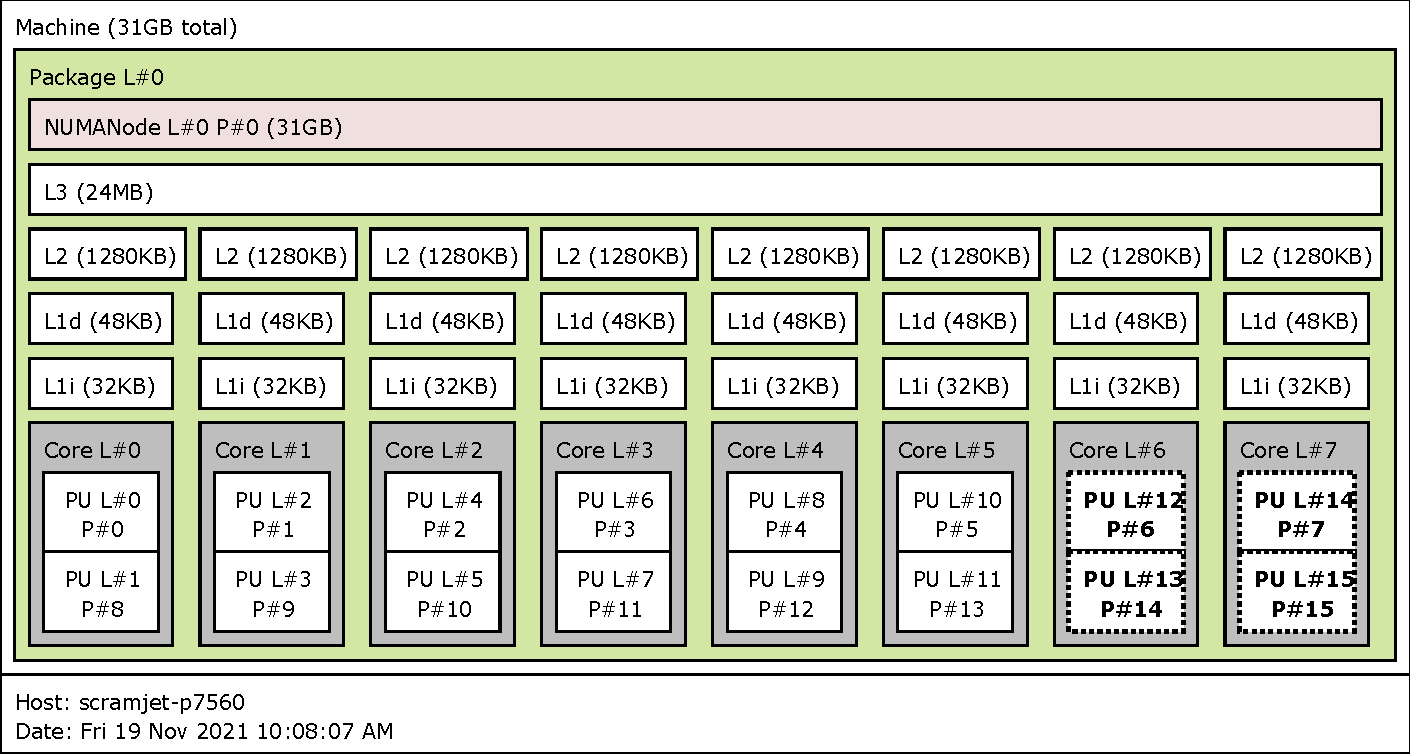
\includegraphics[width=0.8\columnwidth]{images/lstopo.pdf}
	\caption{\texttt{lstopo --no-io} output for 8-core, 16-thread Intel\textsuperscript\textregistered{} Xeon\textsuperscript\textregistered{} W-11955M processor}\label{fig:xeon-lstopo}
\end{figure}

Given the separation of the cores, the problem of \emph{coherence} is encountered: how are accesses (either reads or writes) by one core seen by the others?
These require \emph{coherence protocols}, which dictate the movement and broadcast of accesses from one core to all others.
There are two broad categories of coherence protocols: \emph{snooping}, or \emph{bus-based}, and \emph{directory-based}.
The focus of this experiment will be simulating three snooping protocols: MESI, Dragon, and MOESI, and analysing their performance.

\subsection{Snooping Coherence Protocols}
In snooping protocols, memory accesses by every core are \emph{broadcasted} into a bus.
The cache controllers of all other cores \emph{snoop} on or \emph{listen} to this bus, and change the states of their caches appropriately.
Furthermore, in update-based protocols like Dragon, the bus also provides inter-cache lines, along which updated data may be transmitted.
Each protocol tested in this assignment has different characteristics and optimises for different use-cases (writeback-heavy, inter-cache transfer-heavy).

\subsubsection{MESI Protocol}
MESI is an invalidation-based protocol, containing four states: \textbf{M}odified, \textbf{E}xclusive, \textbf{S}hared, and \textbf{I}nvalid. There are no cache-cache transfers.
As such, all misses for a block are facilitated by accessing the main memory.
A cache accessing a block in the \textbf{M} state in some other cache would have to wait for the latter cache to write back that block to memory, and incur an additional wait penalty.

\begin{figure}[htbp]
	\centering
	\begin{tikzpicture}
		\node[state,initial]	(I) {I};
		\node[state]	(S) [above=2cm of I] {S};
		\node[state]	(E) [above=2cm of S] {E};
		\node[state]	(M) [above=2cm of E] {M};
		\tikzset{font=\scriptsize}
		\path[->] (I) edge [bend left=45] node[rounded corners=3pt,inner sep=1.5pt,fill=white,align=center] {\texttt{PrRd/-}\\\texttt{BusRd(S)}} (S)
		edge [bend left=70] node[rounded corners=3pt,inner sep=1.5pt,fill=white,align=center] {\texttt{PrRd/-}\\\texttt{BusRd(S)}} (E)
		edge [bend left=80] node[rounded corners=3pt,inner sep=1.5pt,fill=white,align=center] {\texttt{PrWr/-}\\\texttt{BusRdX}} (M)
		%
		(S) edge [loop below] node[rounded corners=3pt,align=center] {\texttt{PrRd/-}} ()
		edge [bend left=60] node[rounded corners=3pt,inner sep=1.5pt,fill=white,align=center] {\texttt{PrWr/-}\\\texttt{BusRdX}} (M)
		edge[dotted] [bend left=45] node[rounded corners=3pt,inner sep=1.5pt,fill=white,align=center] {\texttt{BusRdX/}\\\texttt{Flush}} (I)
		%
		(E) edge [loop below] node[rounded corners=3pt,align=center] {\texttt{PrRd/-}} ()
		edge [bend left=45] node[rounded corners=3pt,inner sep=1.5pt,fill=white,align=center] {\texttt{PrWr/-}\\\texttt{BusRdX}} (M)
		edge[dotted] [bend left=45] node[rounded corners=3pt,inner sep=1.5pt,fill=white,align=center] {\texttt{BusRd/-}} (S)
		edge[dotted] [bend left=60] node[rounded corners=3pt,inner sep=1.5pt,fill=white,align=center] {\texttt{BusRdX/Flush}} (I)
		%
		(M) edge [loop below] node[rounded corners=3pt,align=center] {\texttt{PrRd/-}\\\texttt{PrWr/-}} ()
		edge[dotted] [bend left=60] node[rounded corners=3pt,inner sep=1.5pt,fill=white,align=center] {\texttt{BusRd/Flush}} (S)
		edge[dotted] [bend left=80] node[rounded corners=3pt,inner sep=1.5pt,fill=white,align=center] {\texttt{BusRdX/Flush}} (I);
	\end{tikzpicture}
	\caption{MESI protocol states and transitions}\label{fig:mesi-graph}
\end{figure}

\begin{table}[htbp]
	\centering\begin{tabular}{r|cccc}
		           & \textbf{M}                  & \textbf{E}                  & \textbf{S}                  & \textbf{I}                  \\ \hline
		\textbf{M} & \textcolor{red}{\xmark{}}   & \textcolor{red}{\xmark{}}   & \textcolor{red}{\xmark{}}   & \textcolor{green}{\cmark{}} \\
		\textbf{E} & \textcolor{red}{\xmark{}}   & \textcolor{red}{\xmark{}}   & \textcolor{red}{\xmark{}}   & \textcolor{green}{\cmark{}} \\
		\textbf{S} & \textcolor{red}{\xmark{}}   & \textcolor{red}{\xmark{}}   & \textcolor{green}{\cmark{}} & \textcolor{green}{\cmark{}} \\
		\textbf{I} & \textcolor{green}{\cmark{}} & \textcolor{green}{\cmark{}} & \textcolor{green}{\cmark{}} & \textcolor{green}{\cmark{}}
	\end{tabular}
	\caption{Permitted cache states }
	\label{tab:mesi-table}
\end{table}

\cref{fig:mesi-graph} shows the MESI state transition diagram, and \cref{tab:mesi-table} shows valid states between a given pair of cache lines mapping to the same memory block.

\subsubsection{Dragon Protocol}
Dragon is an update-based protocol that drastically improves on MESI, by allowing inter-cache transfers.
There are four states: \textbf{E}xclusive, \textbf{S}hared \textbf{c}lean, \textbf{S}hared \textbf{m}odified, and \textbf{M}odified.
\cref{fig:dragon-graph} depicts the state transitions of the Dragon protocol.
Note that we have additionally implemented the \textbf{I}nvalid state, to represent a clean cache with \emph{no} data whatsoever.

Furthermore, \cref{tab:dragon-table} shows valid states between a given pair of caches mapping to the same memory block, under the Dragon protocol.

\begin{figure}[htbp]
	\centering
	\begin{tikzpicture}% function%\begin{}[]%\\addplot {};%\\end{}%\\end{
		\node[state,initial]	(I) {I};
		\node[state]	(E) [above right=2cm of I] {E};
		\node[state]	(Sm) [below right=2cm of I] {Sm};
		\node[state]	(Sc) [right=4cm of E] {Sc};
		\node[state]	(M) [right=4cm of Sm] {M};s
		\tikzset{font=\scriptsize}
		\path[->] (I) edge node[rounded corners=3pt,inner sep=1.5pt,fill=white,align=center] {\texttt{PrRdMiss}/\\\texttt{BusRd(S')}} (E)
		edge node[rounded corners=3pt,inner sep=1.5pt,fill=white,align=center] {\texttt{PrWrMiss}/\\\texttt{BusRd(S')}} (Sm)
		edge[bend left=100] node[rounded corners=3pt,inner sep=1.5pt,fill=white,align=center] {\texttt{PrRdMiss}/\texttt{BusRd(S)}} (Sc)
		edge[bend right=100] node[rounded corners=3pt,inner sep=1.5pt,fill=white,align=center] {\texttt{PrWrMiss}/\texttt{BusRd(S')}} (M)
		%
		(E) edge node[rounded corners=3pt,align=center,fill=white] {\texttt{BusRd/-}} (Sc)
		edge node[rounded corners=3pt,inner sep=1.5pt,fill=white,align=center] {\texttt{PrWr/-}} (M)
		%
		(Sc) edge [loop right] node[rounded corners=3pt,align=center] {\texttt{PrRd/-}\\\texttt{BusRd/-}\\\texttt{BusUpd/update}} ()
		edge node[rounded corners=3pt,align=center,fill=white] {\texttt{PrWr/}\\\texttt{BusUpd(S')}} (M);
		% edge [bend left=60] node[rounded corners=3pt,inner sep=1.5pt,fill=white,align=center] {\texttt{PrWr/-}\\\texttt{BusRdX}} (M)
		% edge[dotted] [bend left=45] node[rounded corners=3pt,inner sep=1.5pt,fill=white,align=center] {\texttt{BusRdX/}\\\texttt{Flush}} (I)
		% %
		% (M) edge [loop below] node[rounded corners=3pt,align=center] {\texttt{PrRd/-}\\\texttt{PrWr/-}} ()
		% edge[dotted] [bend left=60] node[rounded corners=3pt,inner sep=1.5pt,fill=white,align=center] {\texttt{BusRd/Flush}} (S)
		% edge[dotted] [bend left=80] node[rounded corners=3pt,inner sep=1.5pt,fill=white,align=center] {\texttt{BusRdX/Flush}} (I);
	\end{tikzpicture}
	\caption{Dragon protocol states and transitions}
	\label{fig:dragon-graph}
\end{figure}

\begin{table}[htbp]
	\centering\begin{tabular}{r|cccc}
		            & \textbf{E}                  & \textbf{Sc}                 & \textbf{Sm}                 & \textbf{M}                  \\ \hline
		\textbf{E}  & \textcolor{red}{\xmark{}}   & \textcolor{red}{\xmark{}}   & \textcolor{red}{\xmark{}}   & \textcolor{green}{\xmark{}} \\
		\textbf{Sc} & \textcolor{red}{\xmark{}}   & \textcolor{red}{\cmark{}}   & \textcolor{red}{\cmark{}}   & \textcolor{green}{\xmark{}} \\
		\textbf{Sm} & \textcolor{red}{\xmark{}}   & \textcolor{red}{\cmark{}}   & \textcolor{green}{\xmark{}} & \textcolor{green}{\xmark{}} \\
		\textbf{M}  & \textcolor{green}{\xmark{}} & \textcolor{green}{\xmark{}} & \textcolor{green}{\xmark{}} & \textcolor{green}{\xmark{}}
	\end{tabular}
	\caption{Permitted cache states for MESI}
	\label{tab:dragon-table}
\end{table}

\subsubsection{MOESI Protocol}
The MOESI protocol is similar to the MESI protocol, in that writes cause invalidation to all the other lines in the other
caches.
However, it introduces another state, \textbf{O}wned, that the cache can go into when it encounters a BusRd making it the responsibility
of the owning Cache to sharing the line without writing back to memory.
Hence, unlike the MESI protocol, dirty inter-cache sharing is allowed, which signicantly reduces read latency from 100 (main-memory reads) to 2\(N\) where \(N\) is the number of words, when an owning cache exists.
This drastically reduces the number of main-memory reads in programs that exploit much inter-process communication.
\section{Experimental Design}
\subsection{Programming Language and Build Tools}
Based on our own programming experiences, we had the choices of \Cpp{} and \Cs{}. We chose \Cpp{20} because it allowed us access to several functional libraries like \texttt{<ranges>}.
We also selected it for its speed, given that truly large cache sizes might have needed to be simulated.
Indeed, several configurations of the benchmark took nearly two hours to complete, which might have been far slower had we used \Cs{}.

We also used CMake as a build-generator, so that cross-platform programming could be easily done.
CLion and \texttt{nvim} were used across Windows and Linux to develop the simulator.

\subsection{Design Abstractions and Implementation}
We have chosen an object-oriented design for the simulator, with each component focused on one task.

\subsubsection{Overall System Design}
The \texttt{Runner} class is responsible for accepting input from the command-line, parsing and validating said input, and forwarding it to the \texttt{System} class.
\texttt{Runner} also collects data from the \texttt{CoreMonitor}s and the \texttt{BusMonitor}, prints them to \texttt{stdout} and writes to a \texttt{.csv} file for data analysis.
As such, \texttt{Runner} also contains \texttt{int main()}.

\texttt{System} contains an array of four \texttt{Processor}s, as well as a `smart pointer' (specifically, \texttt{std::unique\textunderscore{}ptr}) to a \texttt{Bus} (or more accurately, one of its derived classes).
Each \texttt{Processor} contains another smart pointer to a \texttt{Cache}, whose ownership is shared by the \texttt{Bus}, so that the latter may update the caches upon any transition being triggered.

\subsubsection{Input Parsing and Validation}
We first check that the number of arguments to the program is correct. At most 5 arguments are expected, and the defaults are used if fewer than 5 arguments are provided.
An exception is thrown if the number of arguments is too high.
Next, we check if the protocols and benchmark names are correct; otherwise, an exception is thrown.
Valid protocol strings are \texttt{"MESI"}, \texttt{"Dragon"}, and \texttt{"MOESI"} (the checks are case-\emph{sensitive}).

Finally, the cache configuration is checked.
The cache size and block size must be some multiple of 4 (the word size), and the cache itself must be a multiple of the block size.
The associativity must then evenly divide the number of blocks, ie the relationship in \cref{eqn:assoc-divide} must be satisfied.
\begin{equation}
	\mathrm{associativity} \equiv 0 \pmod{\text{number of blocks}}\label{eqn:assoc-divide}
\end{equation}
If any of the above conditions fail, the simulator refuses to run, throwing an exception.

\subsubsection{The \texttt{System} Class}
\texttt{System::run()} is the main entry point for the program, and launches a loop that runs indefinitely, as long as any one processor signals that there are still instructions left to process.
This is achieved by setting a member variable appropriately.
In every iteration of the loop, one processor is refreshed, and any blocked cycle counters are decremented.

If a processor is already \emph{not} blocked to begin with, then the \texttt{Bus} triggers state transitions, and the next instruction is streamed in and checked for its type (\texttt{LD}/\texttt{ST}/\texttt{ALU}).
Memory access instructions are then checked against the cache for hits or misses, and the bus transitions all other caches appropriately.

\subsubsection{The \texttt{Processor} Class}
\texttt{Processor} is an abstraction for a system processor. That said, in our implementation, it does little more than provide a convenient container for various counters, the instruction input stream, and the cache itself. The processor

\subsubsection{The \texttt{Bus} Class and Derived Classes}
\texttt{Bus} is an abstract class which calculates the number of cycles the processors need to be blocked for, and also facilitates state transitions for each cache, at the end of the wait period.
The three protocols are implemented as \texttt{MESIBus}, \texttt{DragonBus}, and \texttt{MOESIBus}, which all inherit from a base class, \texttt{Bus}.
This allowed the rest of the components to be agnostic to the currently-running protocol. The derived classes
perform the state transitions based on their respective protocols and also find out the block periods of a cache based on the state of all the caches in case of access misses, based on the protocol.

\texttt{MESIBus} returns a 100 cycle block on any miss, and 1 cycle latency for hits, as no cache to cache sharing is allowed.
\texttt{DragonBus} returns a 2 cycle block for write hits due to word updates, but incurs a 2\(N\) cache latency
for inter-cache block sharing on misses, and a 100 cycle latency if no other cache contains the required information.
\texttt{MOESIBus} forms a middle ground by allowing dirty inter-cache sharing with 2\(N\) cache latency, but returns a 100 cycle block when no other cache contains the block in question.

\subsubsection{The \texttt{Cache} Class}
\texttt{Cache} is our implementation of an \gls{lru} write-back, write-allocate cache.
On each write and read operation, the set containing the block is sorted in the order of the latest-accessed line.
On write misses, the missing block is loaded into the respective set.
Given the \emph{data} itself is not simulated, no modifications are performed, but the state is changed appropriately.

Evictions are picked up by the cache on misses and ejected from the respective set.
Control is then returned to \texttt{Bus}, which then performs a state transition based on the protocol. Writes-back of dirty lines invoke a 100 cycle block.

\subsection{Assumptions Made}
There were a few assumptions we have made in our design of the simulator:
\begin{enumerate}
	\item Instruction fetch and decode takes zero cycles.
	\item There is no pipelining in this simulator: the next instruction is fetched and parsed only when the current instruction has completed running.
	\item Bus transactions are issued \emph{after} data is received, in case of an access miss.
	\item Intermediate bus transactions cause short-circuiting.
	      In other words, suppose a cache A requests block \(x\) at time \(t_1\).
	      Cache B requests the same block at time \(t_2 > t_1\). Our implementation is such that the latter cache would only have to wait for, at a minimum, \(t_2 - t_1\) time before it could access the block.
	      The inter-cache delay is also accounted for, in the case of the Dragon and MOESI protocols.
\end{enumerate}

\section{Results and Analysis}

\ref{legend}

For all the following graphs, we will use the legend above.
We have chosen to plot the miss rate against three independent variables: the cache size, associativity, and the block size.
A Python script was used to run the compiled binary with the appropriate arguments, and more than 7000 inputs were generated.

We have chosen some particular results that clearly depict changes in performance, and the metric we have chosen is the miss rate.
We chose not to use execution time as it is itself dependent on the miss rate (or more particularly, the miss \emph{count}).

\subsection{Cache Size}
\begin{figure}[htbp]
	\centering
	\begin{tikzpicture}
		\pgfplotsset{width=6cm,}
		\begin{axis}[
				xmode=log,log basis x={2},ymode=log,
				title=\texttt{blackscholes},
				legend columns=-1,
				legend entries={MESI, Dragon, MOESI},
				legend style={/tikz/every even column/.append style={column sep=0.5cm}},
				legend to name=legend,
				x tick style={black, thin},
				y tick style={black, thin},
				ticklabel style={font=\footnotesize},
				ymax=1,
				xlabel={Cache size (\si{\byte})},ylabel={Miss rate},
			]
			\addplot[blue,only marks,mark=triangle,] gnuplot[raw gnuplot]{
					set datafile separator ',';
					plot 'csvs/miss_rate_cache_size_blackscholes_MESI.csv' u 15:9;
				};
			\addplot[opacity=0.5,red,only marks,mark=x,] gnuplot[raw gnuplot]{
					set datafile separator ',';
					plot 'csvs/miss_rate_cache_size_blackscholes_Dragon.csv' u 15:9;
				};
			\addplot[opacity=0.4,fill=green,only marks,mark=*,] gnuplot[raw gnuplot]{
					set datafile separator ',';
					plot 'csvs/miss_rate_cache_size_blackscholes_MOESI.csv' u 15:9;
				};
		\end{axis}
	\end{tikzpicture}
	\begin{tikzpicture}
		\pgfplotsset{width=6cm,}
		\begin{axis}[
				xmode=log,log basis x={2},ymode=log,
				title=\texttt{bodytrack},
				legend columns=-1,
				legend entries={MESI, Dragon, MOESI},
				legend style={/tikz/every even column/.append style={column sep=0.5cm}},
				legend to name=legend,
				x tick style={black, thin},
				y tick style={black, thin},
				ticklabel style={font=\footnotesize},
				ymax=1,
				ytick={0.001,0.01,0.1,1},yticklabels={,,},
				% scaled x ticks=base 2,
				xlabel={Cache size (\si{\byte})},
			]
			\addplot[blue,only marks,mark=triangle,] gnuplot[raw gnuplot]{
					set datafile separator ',';
					plot 'csvs/miss_rate_cache_size_bodytrack_MESI.csv' u 15:9;
				};
			\addplot[opacity=0.5,red,only marks,mark=x,] gnuplot[raw gnuplot]{
					set datafile separator ',';
					plot 'csvs/miss_rate_cache_size_bodytrack_Dragon.csv' u 15:9;
				};
			\addplot[opacity=0.4,fill=green,only marks,mark=*,] gnuplot[raw gnuplot]{
					set datafile separator ',';
					plot 'csvs/miss_rate_cache_size_bodytrack_MOESI.csv' u 15:9;
				};
		\end{axis}
	\end{tikzpicture}
	\begin{tikzpicture}
		\pgfplotsset{width=6cm,}
		\begin{axis}[
				xmode=log,log basis x={2},ymode=log,
				title=\texttt{fluidanimate},
				legend columns=-1,
				legend entries={MESI, Dragon, MOESI},
				legend style={/tikz/every even column/.append style={column sep=0.5cm}},
				legend to name=legend,
				x tick style={black, thin},
				y tick style={black, thin},
				ticklabel style={font=\footnotesize},
				ymax=1,
				ytick={0.001,0.01,0.1,1},yticklabels={,,},
				% scaled x ticks=base 2,
				xlabel={Cache size (\si{\byte})},
			]
			\addplot[blue,only marks,mark=triangle,] gnuplot[raw gnuplot]{
					set datafile separator ',';
					plot 'csvs/miss_rate_cache_size_fluidanimate_MESI.csv' u 15:9;
				};
			\addplot[opacity=0.5,red,only marks,mark=x,] gnuplot[raw gnuplot]{
					set datafile separator ',';
					plot 'csvs/miss_rate_cache_size_fluidanimate_Dragon.csv' u 15:9;
				};
			\addplot[opacity=0.4,fill=green,only marks,mark=*,] gnuplot[raw gnuplot]{
					set datafile separator ',';
					plot 'csvs/miss_rate_cache_size_fluidanimate_MOESI.csv' u 15:9;
				};
		\end{axis}
	\end{tikzpicture}
	\caption{Miss rate on cache size, with fixed block size (\SI{32}{\byte}) and 2-way set-associativity}\label{fig:miss_rate_cache_size}
\end{figure}

From \cref{fig:miss_rate_cache_size}, it is obvious that all caches show the same behaviour: increasing the cache size results in a corresponding improvement in performance, as the miss rate decreases from \SI{40}{\percent} to less than \SI{0.5}{\percent} or so.
This improvement is consistent across all three cache protocols.

\subsection{Associativity}
\begin{figure}[htbp]
	\centering
	\begin{tikzpicture}
		\pgfplotsset{width=6cm,}
		\begin{axis}[
				xmode=log,log basis x={2},ymode=log,
				title=\texttt{blackscholes},
				legend columns=-1,
				legend entries={MESI, Dragon, MOESI},
				legend style={/tikz/every even column/.append style={column sep=0.5cm}},
				legend to name=legend,
				x tick style={black, thin},
				y tick style={black, thin},
				ticklabel style={font=\footnotesize},
				ymax=0.1,
				xlabel={Associativity},ylabel={Miss rate},
			]
			\addplot[blue,only marks,mark=triangle,] gnuplot[raw gnuplot]{
					set datafile separator ',';
					plot 'csvs/miss_rate_associativity_blackscholes_MESI.csv' u 16:9;
				};
			\addplot[opacity=0.5,red,only marks,mark=x,] gnuplot[raw gnuplot]{
					set datafile separator ',';
					plot 'csvs/miss_rate_associativity_blackscholes_Dragon.csv' u 16:9;
				};
			\addplot[opacity=0.4,fill=green,only marks,mark=*,] gnuplot[raw gnuplot]{
					set datafile separator ',';
					plot 'csvs/miss_rate_associativity_blackscholes_MOESI.csv' u 16:9;
				};
		\end{axis}
	\end{tikzpicture}
	\begin{tikzpicture}
		\pgfplotsset{width=6cm,}
		\begin{axis}[
				xmode=log,log basis x={2},ymode=log,
				title=\texttt{bodytrack},
				legend columns=-1,
				legend entries={MESI, Dragon, MOESI},
				legend style={/tikz/every even column/.append style={column sep=0.5cm}},
				legend to name=legend,
				x tick style={black, thin},
				y tick style={black, thin},
				ticklabel style={font=\footnotesize},
				ymax=0.1,
				ytick={0.001,0.01,0.1,1},yticklabels={,,},
				xlabel={Associativity},
			]
			\addplot[blue,only marks,mark=triangle,] gnuplot[raw gnuplot]{
					set datafile separator ',';
					plot 'csvs/miss_rate_associativity_bodytrack_MESI.csv' u 16:9;
				};
			\addplot[opacity=0.5,red,only marks,mark=x,] gnuplot[raw gnuplot]{
					set datafile separator ',';
					plot 'csvs/miss_rate_associativity_bodytrack_Dragon.csv' u 16:9;
				};
			\addplot[opacity=0.4,fill=green,only marks,mark=*,] gnuplot[raw gnuplot]{
					set datafile separator ',';
					plot 'csvs/miss_rate_associativity_bodytrack_MOESI.csv' u 16:9;
				};
		\end{axis}
	\end{tikzpicture}
	\begin{tikzpicture}
		\pgfplotsset{width=6cm,}
		\begin{axis}[
				xmode=log,log basis x={2},ymode=log,
				title=\texttt{fluidanimate},
				legend columns=-1,
				legend entries={MESI, Dragon, MOESI},
				legend style={/tikz/every even column/.append style={column sep=0.5cm}},
				legend to name=legend,
				x tick style={black, thin},
				y tick style={black, thin},
				ticklabel style={font=\footnotesize},
				ymax=0.1,
				ytick={0.001,0.01,0.1,1},yticklabels={,,},
				xlabel={Associativity},
			]
			\addplot[blue,only marks,mark=triangle,] gnuplot[raw gnuplot]{
					set datafile separator ',';
					plot 'csvs/miss_rate_associativity_fluidanimate_MESI.csv' u 16:9;
				};
			\addplot[opacity=0.5,red,only marks,mark=x,] gnuplot[raw gnuplot]{
					set datafile separator ',';
					plot 'csvs/miss_rate_associativity_fluidanimate_Dragon.csv' u 16:9;
				};
			\addplot[opacity=0.4,fill=green,only marks,mark=*,] gnuplot[raw gnuplot]{
					set datafile separator ',';
					plot 'csvs/miss_rate_associativity_fluidanimate_MOESI.csv' u 16:9;
				};
		\end{axis}
	\end{tikzpicture}
	\caption{Miss rate on associativity with fixed cache size (\SI{4}{\kibi\byte}) and fixed block size (\SI{32}{\byte})}\label{fig:miss_rate_associativity}
\end{figure}
From \cref{fig:miss_rate_associativity}, it is clear that increasing the associativity of a cache beyond a certain limit provides no real benefit, as diminishing returns are reached.
In the real world, most processor caches do not have associativity counts beyond 8 or 16, as the real limit of compulsory misses is hit.
This means that CPU manufacturers can leave some performance on the table if it means drastically simplified hardware costs.

\subsection{Block Size}
\begin{figure}[htbp]
	\centering
	\begin{tikzpicture}
		\pgfplotsset{width=6cm,}
		\begin{axis}[
				xmode=log,log basis x={2},ymode=log,
				title=\texttt{blackscholes},
				legend columns=-1,
				legend entries={MESI, Dragon, MOESI},
				legend style={/tikz/every even column/.append style={column sep=0.5cm}},
				legend to name=legend,
				x tick style={black, thin},
				y tick style={black, thin},
				ticklabel style={font=\footnotesize},
				ymax=0.1,
				xlabel={Block size (\si{\byte})},ylabel={Miss rate},
			]
			\addplot[blue,only marks,mark=triangle,] gnuplot[raw gnuplot]{
					set datafile separator ',';
					plot 'csvs/miss_rate_line_size_blackscholes_MESI.csv' u 17:9;
				};
			\addplot[opacity=0.5,red,only marks,mark=x,] gnuplot[raw gnuplot]{
					set datafile separator ',';
					plot 'csvs/miss_rate_line_size_blackscholes_Dragon.csv' u 17:9;
				};
			\addplot[opacity=0.4,fill=green,only marks,mark=*,] gnuplot[raw gnuplot]{
					set datafile separator ',';
					plot 'csvs/miss_rate_line_size_blackscholes_MOESI.csv' u 17:9;
				};
		\end{axis}
	\end{tikzpicture}
	\begin{tikzpicture}
		\pgfplotsset{width=6cm,}
		\begin{axis}[
				xmode=log,log basis x={2},ymode=log,
				title=\texttt{bodytrack},
				legend columns=-1,
				legend entries={MESI, Dragon, MOESI},
				legend style={/tikz/every even column/.append style={column sep=0.5cm}},
				legend to name=legend,
				x tick style={black, thin},
				y tick style={black, thin},
				ticklabel style={font=\footnotesize},
				ymax=0.1,
				ytick={0.001,0.01,0.1,1},yticklabels={,,},
				xlabel={Block size (\si{\byte})},
			]
			\addplot[blue,only marks,mark=triangle,] gnuplot[raw gnuplot]{
					set datafile separator ',';
					plot 'csvs/miss_rate_line_size_bodytrack_MESI.csv' u 17:9;
				};
			\addplot[opacity=0.5,red,only marks,mark=x,] gnuplot[raw gnuplot]{
					set datafile separator ',';
					plot 'csvs/miss_rate_line_size_bodytrack_Dragon.csv' u 17:9;
				};
			\addplot[opacity=0.4,fill=green,only marks,mark=*,] gnuplot[raw gnuplot]{
					set datafile separator ',';
					plot 'csvs/miss_rate_line_size_bodytrack_MOESI.csv' u 17:9;
				};
		\end{axis}
	\end{tikzpicture}
	\begin{tikzpicture}
		\pgfplotsset{width=6cm,}
		\begin{axis}[
				xmode=log,log basis x={2},ymode=log,
				title=\texttt{fluidanimate},
				legend columns=-1,
				legend entries={MESI, Dragon, MOESI},
				legend style={/tikz/every even column/.append style={column sep=0.5cm}},
				legend to name=legend,
				x tick style={black, thin},
				y tick style={black, thin},
				ticklabel style={font=\footnotesize},
				ymax=0.1,
				ytick={0.001,0.01,0.1,1},yticklabels={,,},
				xlabel={Block size (\si{\byte})},
			]
			\addplot[blue,only marks,mark=triangle,] gnuplot[raw gnuplot]{
					set datafile separator ',';
					plot 'csvs/miss_rate_line_size_fluidanimate_MESI.csv' u 17:9;
				};
			\addplot[opacity=0.7,red,only marks,mark=x,] gnuplot[raw gnuplot]{
					set datafile separator ',';
					plot 'csvs/miss_rate_line_size_fluidanimate_Dragon.csv' u 17:9;
				};
			\addplot[opacity=0.8,fill=green,only marks,mark=*,] gnuplot[raw gnuplot]{
					set datafile separator ',';
					plot 'csvs/miss_rate_line_size_fluidanimate_MOESI.csv' u 17:9;
				};
		\end{axis}
	\end{tikzpicture}
	\caption{Miss rate on cache line size with fixed cache size (\SI{4}{\kibi\byte}) and 2-way set-associativity}\label{fig:miss_rate_line_size}
\end{figure}
Varying block sizes provide the most interesting results so far, as seen in \cref{fig:miss_rate_line_size}.
Across all caches, miss rates decrease as block sizes increase. There is then a turning point at around \(2^7 \si[]{\byte}\), beyond which miss rates drastically increase with increasing block sizes.
This is because very large block sizes incur big penalties in inter-cache transfers, as the large block needs to be loaded completely on the inter-cache line, and sent to the other caches.
The \texttt{bodytrack} and \texttt{fluidanimate} benchmarks show this behaviour most clearly.

\subsection{Protocols}
From our tests, it is clear that the Dragon protocol outperforms MESI and MOESI in all benchmarks (as expected).
Having zero invalidations with inter-cache sharing (notwithstanding an inconsequential 2 cycle block) allows more lines to be retained, hence reducing the miss rate and significantly boosting performance.
However, this comes at a price: there is heavy bus traffic due to the BusUpdate word shared. In the real world, this might equate to large amounts of heat dissipated on-chip, even if performance is only \emph{acceptable}.

MESI is the worst protocol because it requires writes back for every BusRd.
As already mentioned, there is a default 100-cycle block on writes back, which leads to its poor performance.

Finally, MOESI is an improvement on MESI as dirty inter-cache sharing is allowed. This reduces processor blocks on misses from 100 to 2N in cases when another caches contain a dirty line. Notably, this metric means that there is a point at which \(2N \gg 100\), when it then makes more sense for the caches to write back and then retrieve data from the main memory.
This doesn't reduce the number of invalidations but in large programs, may reduce the overall execution cycles.
However, it still performs worse than Dragon due to the invalidations.
Furthermore, MOESI does not allow for clean line cache to cache sharing.

All that said, if bus traffic were taken into account, this protocol would provide a competitive execution cycle to traffic data ratio compared to Dragon and MESI.@\

\section{Conclusion}
This experiment allowed us to understand and simulate cache coherence, as well as compare their performances.

We confirm the straightforward idea that larger caches lead to increased performance, but associativity only improves performance to a limited extent.
More importantly, we were surprised by the results for block sizes, that led us to further research and justifications for said results.
\end{document}
